\chapter{Introduction}

Unmanned Aerial Systems (UAS) have become a popular platform for both research in academia and civil applications like filming, search and rescue, surveillance, and entertainment. UAS are advantageous for surveillance and target tracking because better visual awareness can be achieved with an airborne camera. Cameras are the most popular sensor on a UAS because of cost, weight, and because they are a rich source of information. For this reason, vision-based target tracking on UAS is an active area of research. This thesis presents some existing control methods as well as novel control schemes for gimbal and UAV in a Visual Servoing context \cite{Hutchinson1996}. 

Visual servoing is another name that is often used to refer to the vision-based robot control. It is a technique to manipulate the robot using information from visual sensors. There are two main types of visual servo control: Position-based visual servo control (PBVS) and Image-based visual servo control (IBVS) \cite{Chaumette2006}. PBVS defines the error in the inertial frame. Thus, PBVS requires reconstructing the 3D inertial coordinates of the feature points from a 2D image. As one can imagine, the reconstructed 3D inertial coordinates can be inaccurate when camera calibration is not done correctly. Another disadvantage of the PBVS, perhaps the most undesirable for the matter that this thesis concerns, is that since the PBVS generates the robot commands in the inertial frame, the objects of interest may leave the camera field of view \cite{Hu2009}. On the other hand, it is important to not lose the target from the camera field of view for tracking application which is the main advantage of the IBVS. In general, IBVS is used to manipulate the robot by calculating the desired servo velocity using image features directly (see Figure \ref{ibvs}). Thus, since this thesis focuses on how to keep a target of interest in sight of a system operator, the IBVS framework fits well with vision-based gimbal control in Chapter \ref{chapter2} and UAV control in Chapter \ref{chapter3}, \ref{chapter4} of this thesis. 

\begin{figure}[htbp]
	\centering
	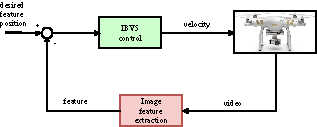
\includegraphics[width = 0.5\textheight]{images/ibvs}
	\caption{Image-based visual servoing (IBVS) structure}
	\label{ibvs}
\end{figure}

Gimbals are widely used device for flying drones with a camera because they stabilize the camera from vibration and movement of the platform. Stabilizing the camera is important in order to take high-quality, smooth videos and photos. For this reason, most of the high-end commercial drones are equipped with a gimbal. For autonomous systems, a gimbal becomes more important because it adds maneuverability to the camera to provide more visual awareness and to keep the object of interest in the camera field of view. There are two cases when the object of interest can be centered on the optical axis. The first is when we know the relative location of the target to the camera. The second is when we know the target location in the image. For many practical applications, it is not feasible to assume that we know the target location in the global frame. Thus, image-based gimbal control is the more practical and realistic way to achieve the goal. In Chapter \ref{chapter2}, we introduce several image-based gimbal control schemes.

Vision-based target tracking has been studied for decades. For example, fixed-wing applications are found in \cite{Saunders2011, Rysdyk2006, Dobrokhodov2006, Qadir2011, Theodorakopoulos2008}, and multirotor applications are in \cite{Pestana2013, Thomas2017, Teuliere2011, Kim2013}. Tracking using a gimbaled camera is studied in \cite{Rysdyk2006, Dobrokhodov2006, Hurak2012}, and tracking with a fixed camera is studied in \cite{Saunders2011, Theodorakopoulos2008, Pestana2013, Thomas2017, Teuliere2011, Kim2013}. However, a common assumption that those studies make is that some information about the target, such as color \cite{Teuliere2011, Kim2013}, shape \cite{Thomas2017} or pattern \cite{Lee2012} is known or provided to the tracking algorithm. Thus, they require the user to specify what to track, or to provide the algorithm with a template image of the target in order for the tracker to be activated. 

For example, the work in \cite{Saunders2011} demonstrates that a target can be kept in the camera field of view by constraining the roll angle of a small fixed-wing UAV in the presence of wind. However, the tracking method uses artificial color information and assumes that the target is static in the world frame. In \cite{Qadir2011}, the tracking algorithm utilizes zero-mean normalized cross correlation to detect and locate the object of interest in the image, and therefore needs to be initialized by the user drawing a box around the target or with a template image of the target. Alternatively, the system described in \cite{Pestana2013} can follow any user specified target in an outdoor environment while the UAS maintains fixed distance to the target using the OpenTLD tracker \cite{Kalal2012}. Occlusions are also well handled due to the machine learning algorithm of the OpenTLD. The advantage of the tracker in \cite{Kalal2012} is that it does not require any previous knowledge about the target of interest and is able to track a great variety of objects. However, the system in \cite{Pestana2013} is strictly designed to track only one target at a time and needs a different tracking framework to extend to the multiple target tracking scenario. Also, the user has to draw a bounding box to initialize the track while trying not to include much of the background. Alternatively, reference \cite{Thomas2017} shows impressive results in following a fast moving target using a receding-horizon control scheme that minimizes the velocity error during the initial transience. Still, the system in \cite{Thomas2017} is limited to detecting and localizing spherical shaped objects of known size. 

The work presented in Chapter \ref{chapter3} overcomes many of these limitations and assumptions by using the recursive random sample consensus (R-RANSAC) algorithm that was first introduced in \cite{Niedfeldt2014} and that was developed to track multiple dynamic targets in clutter. The algorithm has been applied to problems like RADAR tracking \cite{Quist2016, Niedfeldt2014} and UAV Sense and Avoid \cite{Wikle2012}. It has also been applied to vision based scenarios in which R-RANSAC is used to track multiple moving objects from a camera mounted on both static and mobile platforms \cite{Ingersoll2015, Defranco2015}. Chapter \ref{chapter3} extends our previous work and is the first attempt to close the feedback loop of a UAS around the R-RANSAC vision based tracking algorithm. The system presented here is unique in terms of tracking multiple objects that are in the camera field of view. Also, through the hardware demonstration, it is validated that the system can track realistic targets in unstructured environments with satisfactory performance. All operations in the hardware results are autonomous except for selecting the desired target ID.

The control law presented in Chapter \ref{chapter3} is relatively simple and has limitation. It can only compute the desired UAV position when the target is moving on a flat surface and when the correct UAV altitude is available. Thus, Chapter \ref{chapter4} introduces new control algorithm to overcome the limitation by incorporating adaptive control and backstepping control techniques. With mathematical derivation and simulation result, this algorithm is promising to be used in target tracking situation when the target is moving on unleveled surface. Testing the algorithm with hardware remains as future work. 

Lastly, Chapter \ref{chapter5} provides a brief summary of the main contents and gives some suggestions and recommendations for the future work that can extend what has been done in this research. 

The main contributions of this thesis are
\begin{enumerate}
	\item presenting three gimbal control algorithms including newly developed adaptive depth gimbal control.
	\item integrating the system for multirotor autonomous target following using Recursive-RANSAC tracker and demonstrating the hardware results.
	\item developing the unit vector visual servoing framework for UAV control in target tracking.
\end{enumerate}